% Options for packages loaded elsewhere
\PassOptionsToPackage{unicode}{hyperref}
\PassOptionsToPackage{hyphens}{url}
%
\documentclass[
]{article}
\usepackage{amsmath,amssymb}
\usepackage{lmodern}
\usepackage{iftex}
\ifPDFTeX
  \usepackage[T1]{fontenc}
  \usepackage[utf8]{inputenc}
  \usepackage{textcomp} % provide euro and other symbols
\else % if luatex or xetex
  \usepackage{unicode-math}
  \defaultfontfeatures{Scale=MatchLowercase}
  \defaultfontfeatures[\rmfamily]{Ligatures=TeX,Scale=1}
\fi
% Use upquote if available, for straight quotes in verbatim environments
\IfFileExists{upquote.sty}{\usepackage{upquote}}{}
\IfFileExists{microtype.sty}{% use microtype if available
  \usepackage[]{microtype}
  \UseMicrotypeSet[protrusion]{basicmath} % disable protrusion for tt fonts
}{}
\makeatletter
\@ifundefined{KOMAClassName}{% if non-KOMA class
  \IfFileExists{parskip.sty}{%
    \usepackage{parskip}
  }{% else
    \setlength{\parindent}{0pt}
    \setlength{\parskip}{6pt plus 2pt minus 1pt}}
}{% if KOMA class
  \KOMAoptions{parskip=half}}
\makeatother
\usepackage{xcolor}
\IfFileExists{xurl.sty}{\usepackage{xurl}}{} % add URL line breaks if available
\IfFileExists{bookmark.sty}{\usepackage{bookmark}}{\usepackage{hyperref}}
\hypersetup{
  pdftitle={Adjusted Limited Dependent Variable Mixture Models of Health State Utilities in R},
  pdfauthor={Mark Pletscher},
  hidelinks,
  pdfcreator={LaTeX via pandoc}}
\urlstyle{same} % disable monospaced font for URLs
\usepackage[margin=1in]{geometry}
\usepackage{color}
\usepackage{fancyvrb}
\newcommand{\VerbBar}{|}
\newcommand{\VERB}{\Verb[commandchars=\\\{\}]}
\DefineVerbatimEnvironment{Highlighting}{Verbatim}{commandchars=\\\{\}}
% Add ',fontsize=\small' for more characters per line
\usepackage{framed}
\definecolor{shadecolor}{RGB}{248,248,248}
\newenvironment{Shaded}{\begin{snugshade}}{\end{snugshade}}
\newcommand{\AlertTok}[1]{\textcolor[rgb]{0.94,0.16,0.16}{#1}}
\newcommand{\AnnotationTok}[1]{\textcolor[rgb]{0.56,0.35,0.01}{\textbf{\textit{#1}}}}
\newcommand{\AttributeTok}[1]{\textcolor[rgb]{0.77,0.63,0.00}{#1}}
\newcommand{\BaseNTok}[1]{\textcolor[rgb]{0.00,0.00,0.81}{#1}}
\newcommand{\BuiltInTok}[1]{#1}
\newcommand{\CharTok}[1]{\textcolor[rgb]{0.31,0.60,0.02}{#1}}
\newcommand{\CommentTok}[1]{\textcolor[rgb]{0.56,0.35,0.01}{\textit{#1}}}
\newcommand{\CommentVarTok}[1]{\textcolor[rgb]{0.56,0.35,0.01}{\textbf{\textit{#1}}}}
\newcommand{\ConstantTok}[1]{\textcolor[rgb]{0.00,0.00,0.00}{#1}}
\newcommand{\ControlFlowTok}[1]{\textcolor[rgb]{0.13,0.29,0.53}{\textbf{#1}}}
\newcommand{\DataTypeTok}[1]{\textcolor[rgb]{0.13,0.29,0.53}{#1}}
\newcommand{\DecValTok}[1]{\textcolor[rgb]{0.00,0.00,0.81}{#1}}
\newcommand{\DocumentationTok}[1]{\textcolor[rgb]{0.56,0.35,0.01}{\textbf{\textit{#1}}}}
\newcommand{\ErrorTok}[1]{\textcolor[rgb]{0.64,0.00,0.00}{\textbf{#1}}}
\newcommand{\ExtensionTok}[1]{#1}
\newcommand{\FloatTok}[1]{\textcolor[rgb]{0.00,0.00,0.81}{#1}}
\newcommand{\FunctionTok}[1]{\textcolor[rgb]{0.00,0.00,0.00}{#1}}
\newcommand{\ImportTok}[1]{#1}
\newcommand{\InformationTok}[1]{\textcolor[rgb]{0.56,0.35,0.01}{\textbf{\textit{#1}}}}
\newcommand{\KeywordTok}[1]{\textcolor[rgb]{0.13,0.29,0.53}{\textbf{#1}}}
\newcommand{\NormalTok}[1]{#1}
\newcommand{\OperatorTok}[1]{\textcolor[rgb]{0.81,0.36,0.00}{\textbf{#1}}}
\newcommand{\OtherTok}[1]{\textcolor[rgb]{0.56,0.35,0.01}{#1}}
\newcommand{\PreprocessorTok}[1]{\textcolor[rgb]{0.56,0.35,0.01}{\textit{#1}}}
\newcommand{\RegionMarkerTok}[1]{#1}
\newcommand{\SpecialCharTok}[1]{\textcolor[rgb]{0.00,0.00,0.00}{#1}}
\newcommand{\SpecialStringTok}[1]{\textcolor[rgb]{0.31,0.60,0.02}{#1}}
\newcommand{\StringTok}[1]{\textcolor[rgb]{0.31,0.60,0.02}{#1}}
\newcommand{\VariableTok}[1]{\textcolor[rgb]{0.00,0.00,0.00}{#1}}
\newcommand{\VerbatimStringTok}[1]{\textcolor[rgb]{0.31,0.60,0.02}{#1}}
\newcommand{\WarningTok}[1]{\textcolor[rgb]{0.56,0.35,0.01}{\textbf{\textit{#1}}}}
\usepackage{longtable,booktabs,array}
\usepackage{calc} % for calculating minipage widths
% Correct order of tables after \paragraph or \subparagraph
\usepackage{etoolbox}
\makeatletter
\patchcmd\longtable{\par}{\if@noskipsec\mbox{}\fi\par}{}{}
\makeatother
% Allow footnotes in longtable head/foot
\IfFileExists{footnotehyper.sty}{\usepackage{footnotehyper}}{\usepackage{footnote}}
\makesavenoteenv{longtable}
\usepackage{graphicx}
\makeatletter
\def\maxwidth{\ifdim\Gin@nat@width>\linewidth\linewidth\else\Gin@nat@width\fi}
\def\maxheight{\ifdim\Gin@nat@height>\textheight\textheight\else\Gin@nat@height\fi}
\makeatother
% Scale images if necessary, so that they will not overflow the page
% margins by default, and it is still possible to overwrite the defaults
% using explicit options in \includegraphics[width, height, ...]{}
\setkeys{Gin}{width=\maxwidth,height=\maxheight,keepaspectratio}
% Set default figure placement to htbp
\makeatletter
\def\fps@figure{htbp}
\makeatother
\setlength{\emergencystretch}{3em} % prevent overfull lines
\providecommand{\tightlist}{%
  \setlength{\itemsep}{0pt}\setlength{\parskip}{0pt}}
\setcounter{secnumdepth}{5}
\ifLuaTeX
  \usepackage{selnolig}  % disable illegal ligatures
\fi
\newlength{\cslhangindent}
\setlength{\cslhangindent}{1.5em}
\newlength{\csllabelwidth}
\setlength{\csllabelwidth}{3em}
\newenvironment{CSLReferences}[2] % #1 hanging-ident, #2 entry spacing
 {% don't indent paragraphs
  \setlength{\parindent}{0pt}
  % turn on hanging indent if param 1 is 1
  \ifodd #1 \everypar{\setlength{\hangindent}{\cslhangindent}}\ignorespaces\fi
  % set entry spacing
  \ifnum #2 > 0
  \setlength{\parskip}{#2\baselineskip}
  \fi
 }%
 {}
\usepackage{calc}
\newcommand{\CSLBlock}[1]{#1\hfill\break}
\newcommand{\CSLLeftMargin}[1]{\parbox[t]{\csllabelwidth}{#1}}
\newcommand{\CSLRightInline}[1]{\parbox[t]{\linewidth - \csllabelwidth}{#1}\break}
\newcommand{\CSLIndent}[1]{\hspace{\cslhangindent}#1}

\title{Adjusted Limited Dependent Variable Mixture Models of Health State Utilities in R}
\author{Mark Pletscher\footnote{Institute of Health Economics and Health Policy, Bern University of Applied Sciences, \href{mailto:mark.pletscher@bfh.ch}{\nolinkurl{mark.pletscher@bfh.ch}}}}
\date{2021-06-25}

\begin{document}
\maketitle

\hypertarget{introduction}{%
\section{Introduction}\label{introduction}}

Health-related quality of life is a key outcome in health technology assessments because it is patient-relevant and it is needed to calculate quality-adjusted life years. Quality of life instruments typically measure health problems in multiple domains using ordinal Likert scales. Value sets or valuation functions convert these profiles of ordinal measures into cardinal health-related utilities between 1 (perfect health) and minus infinity, where 0 represents death, and negative values represent health states worse than death. Because 100\% quality of life represents perfect health, health state utilities are limited at 1. The lowest possible utility in a local value set further defines a lower limit of health state utilities in a local population. Thus, health state utilities are limited dependent variables. In addition, health state utilities often show gaps between 1 and the next smaller utility in the value set. These gaps occur more frequently in quality of life instruments with few levels in the Likert scales such as the EQ-5D-3L (Mulhern et al. 2018). A last but important particularity of health state utilities is that they can be the consequence of multiple latent classes, or they can exhibit multi-modal marginal densities (Hernández Alava et al. 2014).

Adjusted limited dependent variable mixture models are finite mixtures of normal distributions that account for limits, gaps between 1 and the next smaller utility value and multi-modality (Hernández Alava, Wailoo, and Ara 2012; Hernández Alava et al. 2013, 2014; Hernández Alava and Wailoo 2015; Mukuria et al. 2019). These features can improve empirical fit, parameter identification and predictive accuracy compared to standard regression models. Thus, adjusted limited dependent variable mixture models are particularly useful for mapping studies (Gray, Wailoo, and Alava 2018; Gray, Alava, and Wailoo 2018; Dixon, Hollingworth, and Sparrow 2020; Yang et al. 2019; Xu et al. 2020; Fuller et al. 2017; Pennington et al. 2020) but can also improve the identification of incremental and average marginal effects of medical interventions or health problems (e.g. Hvidberg (2016)).

The R `aldvmm' package is an implementation of the adjusted limited dependent variable model mixture model proposed by Hernández Alava and Wailoo (2015) using normal component distributions and a multinomial logit model of probabilities of component membership.

The objectives of this vignette are to demonstrate the usage of the `aldvmm' package, show important challenges of fitting adjusted limited dependent variable mixture models and validate the R implementation against the STATA\textsuperscript{\textregistered} package (Hernández Alava and Wailoo 2015) using publicly available data.

\hypertarget{methods}{%
\section{Methods}\label{methods}}

Adjusted limited dependent variable mixture models are finite mixtures of normal distributions in \(K\) components \(c\) with conditional expectations \(E[y|X, c] = X\beta^{c}\) and standard deviations \(\sigma^{c}\). The probabilities of component membership are estimated using a multinomial logit model as \(P[c|X]=exp(X\delta^{c})/\sum_{k=1}^{K}exp(X\delta^{k})\). The model accumulates the density mass of the finite mixture below a minimum value \(\Psi_1\) at the value \(\Psi_1\), and the density mass above a maximum value \(\Psi_{2}\) at 1. If the maximum value \(\Psi_2\) is smaller than 1, the model emulates a value set with a gap between 1 and the next smaller value.

\begin{equation}
\label{eq:limits}
\begin{array}{ll}
y_{i}|c =& \begin{cases} \begin{array}{ll}
1        & \text{if } y_{i}|c > \Psi_{2}\\
\Psi_{1} & \text{if } y_{i}|c \leq \Psi_{1}\\
y_{i}|c  & \text{if } \Psi_{1} < y_{i}|c \leq \Psi_{2}\\
\end{array} \end{cases}
\end{array}
\end{equation}

In this vignette, we estimate the same models of post-operative EQ-5D-3L utilities as Hernández Alava and Wailoo (2015) and include post-operative Oxford Hip Scores (divided by 10) as the only explanatory variable \(x\).

\begin{equation}
\label{eq:models}
\begin{array}{lrl}
\text{Model 1:}& E[y|c, X] &= \beta_{0}^{c} + \beta_{1}^{c}x\\
& P[c|X]    &= \text{mlogit}(\delta_{0}^{c})\\
&&\\
\text{Model 2:}& E[y|c, X] &= \beta_{0}^{c}  + \beta_{1}^{c}x\\
& P[c|X]    &= \text{mlogit}(\delta_{0}^{c} + \delta_{1}^{c}x)
\end{array}
\end{equation}

The aldvmm() function fits an adjusted limited dependent variable mixture model using the likelihood function from Hernández Alava and Wailoo (2015). The function calls optimr::optimr to minimize the negative log-likelihood using numerical gradients from numDeriv::grad(). The aldvmm() function accepts all optimization methods available in optimr::optimr() except for ``nlm,'' which requires a different implementation of the likelihood function.

The model formula in aldvmm() is an object of class ``formula'' with two parts on the right-hand side of \(\sim\). The first part on the left of the \textbar{} delimiter represents the model of expected values of \(K\) normal distributions. The second part on the right of the \textbar{} delimiter represents the model of probabilities of component membership from a multinomial logit model.

The `aldvmm' package provides four options for the generation of starting values of the optimization algorithm.

\begin{enumerate}
\def\labelenumi{\arabic{enumi}.}
\item
  ``zero'': A vector of zeroes (default).
\item
  ``random'': A vector of standard normal random values.
\item
  ``constant'': Parameter estimates of a constant-only model as starting values for intercepts and standard deviations, and zeroes for all other parameters.\footnote{The auxiliary models for obtaining starting values are fitted using zero starting values.}
\item
  ``sann'': Parameter estimates of a simulated annealing algorithm.
\end{enumerate}

The `aldvmm' package obtains fitted values using the expected value function from Hernández Alava and Wailoo (2015). Covariance matrices and standard errors of parameters are obtained from a numerical approximation of the hessian matrix using numDeriv::hessian(). Standard errors of fitted values in the estimation data \(SE^{fit}_{i}\) and standard errors of predicted values in new data \(SE^{pred}_{i}\) are calculated using the delta method (Dowd, Greene, and Norton 2014; Whitmore 1986). \(G_{i}\) denotes the gradient of a fitted value with respect to changes in parameter estimates, \(\Sigma\) denotes the covariance matrix of parameters, and \(MSE\) denotes the mean squared error of fitted versus observed values in the estimation data.
\begin{equation}
\begin{array}{rl}
SE^{fit}_{i} &= \sqrt{G_{i}'\Sigma G_{i}}
\end{array}
\end{equation}
\begin{equation}
\begin{array}{rl}
SE^{pred}_{i} &= \sqrt{MSE + G_{i}'\Sigma G_{i}}
\end{array}
\end{equation}

The aldvmm() function returns an object of S3 class ``aldvmm'' for which methods for generic functions summary() and predict() are available.

\hypertarget{installation}{%
\section{Installation}\label{installation}}

The `aldvmm' package can be installed from github using the function install\_github() from the `devtools' package.

\begin{Shaded}
\begin{Highlighting}[]
\CommentTok{\# install.packages("devtools")}
\NormalTok{devtools}\SpecialCharTok{::}\FunctionTok{install\_github}\NormalTok{(}\StringTok{"pletschm/aldvmm"}\NormalTok{, }\AttributeTok{ref =} \StringTok{"main"}\NormalTok{)}
\end{Highlighting}
\end{Shaded}

\hypertarget{data}{%
\section{Data}\label{data}}

We analyze the same publicly available \href{https://digital.nhs.uk/data-and-information/publications/statistical/patient-reported-outcome-measures-proms/finalised-patient-reported-outcome-measures-proms-in-england-april-2011-to-march-2012}{\(\text{\underline{EQ-5D-3L utility data}}\)} from English patients after hip replacement in 2011 and 2012 (NHS Digital 2013) as Hernández Alava and Wailoo (2015) in their description of the STATA\textsuperscript{\textregistered} ALDVMM package.

\begin{Shaded}
\begin{Highlighting}[]
\NormalTok{temp }\OtherTok{\textless{}{-}} \FunctionTok{tempfile}\NormalTok{()}

\NormalTok{url }\OtherTok{\textless{}{-}} \FunctionTok{paste0}\NormalTok{(}\StringTok{"https://files.digital.nhs.uk/publicationimport/pub11xxx/"}\NormalTok{,}
              \StringTok{"pub11359/final{-}proms{-}eng{-}apr11{-}mar12{-}data{-}pack{-}csv.zip"}\NormalTok{)}

\FunctionTok{download.file}\NormalTok{(url, temp)}
\FunctionTok{rm}\NormalTok{(url)}

\NormalTok{df }\OtherTok{\textless{}{-}} \FunctionTok{read.table}\NormalTok{(}\FunctionTok{unz}\NormalTok{(}\AttributeTok{description =}\NormalTok{ temp,}
                     \AttributeTok{filename =} \StringTok{"Hip Replacement 1112.csv"}\NormalTok{),}
                 \AttributeTok{sep =} \StringTok{","}\NormalTok{,}
                 \AttributeTok{header =} \ConstantTok{TRUE}\NormalTok{)}

\FunctionTok{unlink}\NormalTok{(temp)}
\FunctionTok{rm}\NormalTok{(temp)}

\NormalTok{df }\OtherTok{\textless{}{-}}\NormalTok{ df[, }\FunctionTok{c}\NormalTok{(}\StringTok{"AGEBAND"}\NormalTok{, }\StringTok{"SEX"}\NormalTok{, }\StringTok{"Q2\_EQ5D\_INDEX"}\NormalTok{, }\StringTok{"HR\_Q2\_SCORE"}\NormalTok{)]}
\NormalTok{df }\OtherTok{\textless{}{-}}\NormalTok{ df[df}\SpecialCharTok{$}\NormalTok{AGEBAND }\SpecialCharTok{!=} \StringTok{"*"} \SpecialCharTok{\&}\NormalTok{ df}\SpecialCharTok{$}\NormalTok{SEX }\SpecialCharTok{!=} \StringTok{"*"}\NormalTok{, ]}

\NormalTok{df}\SpecialCharTok{$}\NormalTok{eq5d }\OtherTok{\textless{}{-}}\NormalTok{ df}\SpecialCharTok{$}\NormalTok{Q2\_EQ5D\_INDEX}
\NormalTok{df}\SpecialCharTok{$}\NormalTok{hr }\OtherTok{\textless{}{-}}\NormalTok{ df}\SpecialCharTok{$}\NormalTok{HR\_Q2\_SCORE}\SpecialCharTok{/}\DecValTok{10}

\NormalTok{df }\OtherTok{\textless{}{-}}\NormalTok{ df[stats}\SpecialCharTok{::}\FunctionTok{complete.cases}\NormalTok{(df), ]}

\FunctionTok{set.seed}\NormalTok{(}\DecValTok{101010101}\NormalTok{)}
\NormalTok{df }\OtherTok{\textless{}{-}}\NormalTok{ df[}\FunctionTok{sample}\NormalTok{(}\DecValTok{1}\SpecialCharTok{:}\FunctionTok{nrow}\NormalTok{(df), }\AttributeTok{size =} \FunctionTok{nrow}\NormalTok{(df)}\SpecialCharTok{*}\FloatTok{0.3}\NormalTok{), ]}
\end{Highlighting}
\end{Shaded}

The data includes 35'166 observations with complete information on patients' post-operative utilities, Oxford Hip Scores, age and sex. Like Hernández Alava and Wailoo (2015), we draw a 30\% sub-sample of 10'549 observations from the population of complete observations of these variables. Although we follow the same approach as Hernández Alava and Wailoo (2015) in the preparation of the data, our random sample is not identical to the data used in their study. Post-operative EQ-5D-3L utilities from English value sets (Dolan 1997) show a bimodal distribution, limits at -0.594 and 1 and a gap between 1 and 0.883 (figure \ref{fig:plot-hist-obs}).

\begin{figure}
\centering
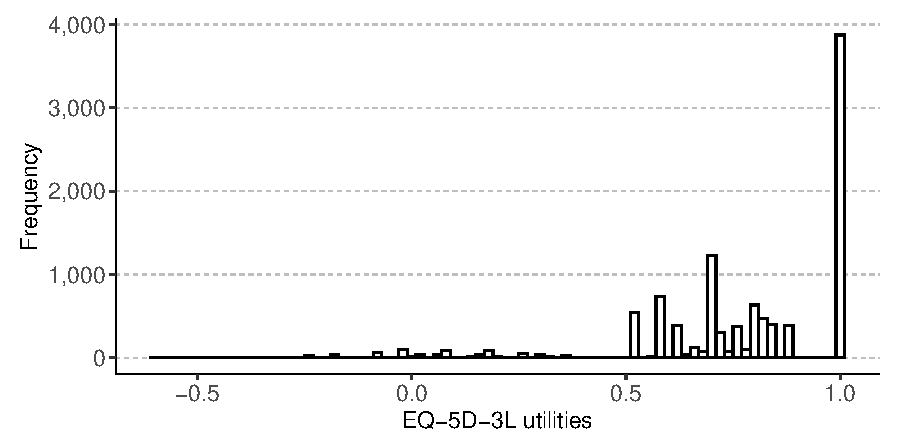
\includegraphics{aldvmm_vignette_files/figure-latex/plot-hist-obs-1.pdf}
\caption{\label{fig:plot-hist-obs}Frequency distribtution of observed EQ-5D-3L utilities}
\end{figure}

\hypertarget{results}{%
\section{Results}\label{results}}

\hypertarget{model-1}{%
\subsection{Model 1}\label{model-1}}

\hypertarget{sec:base}{%
\subsubsection{BFGS optimization method with zero-only starting values}\label{sec:base}}

We first fit model 1 with the ``BFGS'' optimization method and ``zero'' initial values. The values 0.883 and -0.594 in the argument `psi' represent the maximum and minimum values smaller than 1 in the English value set (Dolan 1997). As the data showed a bi-modal distribution (figure \ref{fig:plot-hist-obs}), we estimate a mixture of 2 normal distributions (`ncmp' = 2). aldvmm() returns an object of class ``aldvmm.''

\begin{Shaded}
\begin{Highlighting}[]
\FunctionTok{library}\NormalTok{(}\StringTok{"aldvmm"}\NormalTok{)}

\NormalTok{fit }\OtherTok{\textless{}{-}}\NormalTok{ aldvmm}\SpecialCharTok{::}\FunctionTok{aldvmm}\NormalTok{(eq5d }\SpecialCharTok{\textasciitilde{}}\NormalTok{ hr }\SpecialCharTok{|} \DecValTok{1}\NormalTok{,}
                      \AttributeTok{data =}\NormalTok{ df,}
                      \AttributeTok{psi =} \FunctionTok{c}\NormalTok{(}\FloatTok{0.883}\NormalTok{, }\SpecialCharTok{{-}}\FloatTok{0.594}\NormalTok{),}
                      \AttributeTok{ncmp =} \DecValTok{2}\NormalTok{,}
                      \AttributeTok{init.method =} \StringTok{"zero"}\NormalTok{,}
                      \AttributeTok{optim.method =} \StringTok{"BFGS"}\NormalTok{)}

\FunctionTok{summary}\NormalTok{(fit)}

\NormalTok{pred }\OtherTok{\textless{}{-}} \FunctionTok{predict}\NormalTok{(fit,}
                \AttributeTok{newdata =}\NormalTok{ df,}
                \AttributeTok{se.fit =} \ConstantTok{TRUE}\NormalTok{,}
                \AttributeTok{type =} \StringTok{"fit"}\NormalTok{)}
\end{Highlighting}
\end{Shaded}

We obtain a summary table of regression results using the generic function summary(). The model converges at a log-likelihood of 706.32 and an Akaike information criterion value of -1'398.65 (table \ref{tab:tab-sum-mod1bfgs}).

The coefficients of the intercept and covariates for the expected values \(E[y|c, X]\) of the normal distributions can be interpreted as marginal effects on component means. `lnsigma' denotes the natural logarithm of the estimated standard deviation \(\sigma^{c}\). The coefficients of covariates in the multinomial logit model of probabilities of component membership are log-transformed relative probabilities. Our model only includes two components, and the multinomial logit model collapses to a binomial logit model. The intercept of 0.728 means that the average probability of an observation in the data to belong to component 1 is \(\text{exp}(0.728)\) or 2.0709346 times the probability to belong to component 2.

\begin{table}[ht]
\centering
\caption{Regression results from model1 with "BFGS" optimization method and "zero" starting values} 
\label{tab:tab-sum-mod1bfgs}
\begin{tabular}{llrrrrrr}
  \hline
 &  & Estimate & Std. Err. & z & P$>$$|$z$|$ & [95\% Conf.  & Interval] \\ 
  \hline
E[y$|$X, c] &  &  &  &  &  &  &  \\ 
   \hline
Comp1 & (Intercept) & 0.236 & 0.007 & 34.179 & 0.000 & 0.222 & 0.249 \\ 
   & hr & 0.146 & 0.002 & 76.362 & 0.000 & 0.142 & 0.150 \\ 
   & lnsigma & -2.462 & 0.018 & -138.131 & 0.000 & -2.497 & -2.427 \\ 
  Comp2 & (Intercept) & -0.431 & 0.022 & -19.231 & 0.000 & -0.475 & -0.387 \\ 
   & hr &  0.313 & 0.007 &  47.942 & 0.000 &  0.301 &  0.326 \\ 
   & lnsigma & -1.248 & 0.022 & -57.989 & 0.000 & -1.290 & -1.206 \\ 
   \hline
P[c$|$X] &  &  &  &  &  &  &  \\ 
   \hline
Comp1 & (Intercept) & 0.728 & 0.061 & 12.006 & 0.000 & 0.609 & 0.847 \\ 
   \hline
N = 10549 & ll = 706.32 & AIC = -1398.65 & BIC = -1398.65 &  &  &  &  \\ 
  \end{tabular}
\end{table}

We obtain expected values of observations in the estimation data using the generic function predict(). Standard errors of fitted (estimation data) or predicted (new data) values are calculated using the delta method. Expected values exhibit a smoother distribution than observed values and do not show a gap between 1 and 0.883, because they are weighted averages of component distributions and 1.

\begin{figure}
\centering
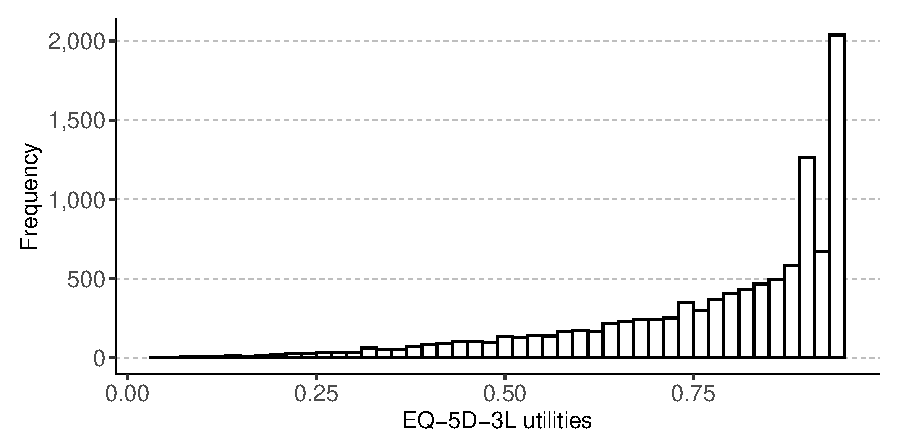
\includegraphics{aldvmm_vignette_files/figure-latex/plot-hist-pred-1.pdf}
\caption{\label{fig:plot-hist-pred}Expected values from base case model}
\end{figure}

\hypertarget{comparison-of-optimization-methods}{%
\subsubsection{Comparison of optimization methods}\label{comparison-of-optimization-methods}}

Hernández Alava and Wailoo (2015) suggested that the likelihood function of the adjusted limited dependent variable mixture model with the English EQ-5D-3L data might have multiple local optima, and that the estimation is sensitive to initial values. We thus fit model 1 with all optimization algorithms and methods for generating initial values available in aldvmm() to assess the sensitivity of the model to optimization settings and to find the maximum likelihood estimates.

\begin{Shaded}
\begin{Highlighting}[]
\NormalTok{init.method }\OtherTok{\textless{}{-}} \FunctionTok{c}\NormalTok{(}\StringTok{"zero"}\NormalTok{, }\StringTok{"random"}\NormalTok{, }\StringTok{"constant"}\NormalTok{, }\StringTok{"sann"}\NormalTok{)}

\NormalTok{optim.method }\OtherTok{\textless{}{-}} \FunctionTok{c}\NormalTok{(}\StringTok{"Nelder{-}Mead"}\NormalTok{, }\StringTok{"BFGS"}\NormalTok{, }\StringTok{"CG"}\NormalTok{, }\StringTok{"L{-}BFGS{-}B"}\NormalTok{, }\StringTok{"nlminb"}\NormalTok{, }\StringTok{"Rcgmin"}\NormalTok{, }
                  \StringTok{"Rvmmin"}\NormalTok{,}\StringTok{"hjn"}\NormalTok{)}

\NormalTok{fit1\_all }\OtherTok{\textless{}{-}} \FunctionTok{list}\NormalTok{()}

\ControlFlowTok{for}\NormalTok{ (i }\ControlFlowTok{in}\NormalTok{ init.method) \{}
  \ControlFlowTok{for}\NormalTok{ (j }\ControlFlowTok{in}\NormalTok{ optim.method) \{}
    \FunctionTok{set.seed}\NormalTok{(}\DecValTok{101010101}\NormalTok{) }\CommentTok{\# Seed for random starting values}
\NormalTok{    fit1\_all[[i]][[j]] }\OtherTok{\textless{}{-}}\NormalTok{ aldvmm}\SpecialCharTok{::}\FunctionTok{aldvmm}\NormalTok{(eq5d }\SpecialCharTok{\textasciitilde{}}\NormalTok{ hr }\SpecialCharTok{|} \DecValTok{1}\NormalTok{,}
                                         \AttributeTok{data         =}\NormalTok{ df,}
                                         \AttributeTok{psi          =} \FunctionTok{c}\NormalTok{(}\FloatTok{0.883}\NormalTok{, }\SpecialCharTok{{-}}\FloatTok{0.594}\NormalTok{),}
                                         \AttributeTok{ncmp         =} \DecValTok{2}\NormalTok{,}
                                         \AttributeTok{init.method  =}\NormalTok{ i,}
                                         \AttributeTok{optim.method =}\NormalTok{ j)}
\NormalTok{  \}}
\NormalTok{\}}
\end{Highlighting}
\end{Shaded}

The maximum likelihood varies considerably across optimization methods and initial values which confirms the sensitivity of the model to changes in these settings (table \ref{tab:ll}). The most frequent log-likelihood is 706.32, but the Hooke and Jeeves Pattern Search Optimization (``hjn'') with ``zero'' initial values converges at a log-likelihood 33'057.43.

The optimization methods ``Nelder-Mead,'' ``CG,'' ``L-BFGS-B,'' and ``Rvmmin'' are particularly sensitive to starting values. The method ``BFGS'' coverges at a log-likelihood of 706.32 with three of four sets of initial values, and the method ``hjn'' with two of four sets of initial values. The methods ``nlminb'' and ``Rcgmin'' converge at a log-likelihood of 706.32 regardless of initial values.

\begin{table}[ht]
\centering
\caption{Log-likelihood by optimization method} 
\label{tab:ll}
\begin{tabular}{lrrrrrrrr}
  \hline
 & Nelder-Mead & BFGS & CG & L-BFGS-B & nlminb & Rcgmin & Rvmmin & hjn \\ 
  \hline
zero & -259.21 & 706.32 & 223.96 & -4513.33 & 706.32 & 706.32 & -8393.14 & 33057.43 \\ 
  random & -434.21 & -623.98 & 65.03 & -2830.18 & 706.32 & 706.32 & -11074.58 & -627.78 \\ 
  constant & 354.36 & 706.32 & -601.52 & -634.81 & 706.32 & 706.32 & -10867.67 & 706.32 \\ 
  sann & 706.19 & 706.32 & 576.51 & 706.32 & 706.32 & 706.32 & 706.32 & 706.32 \\ 
   \hline
\end{tabular}
\end{table}

The computation times of optimization routines vary considerably across methods (table \ref{tab:time}). The optimization methods ``Nelder-Mead,'' ``BFGS,'' ``L-BFGS-B'' and ``Rvmmin'' are the fastest methods, but this speed comes at the cost of a higher risk of convergence at local optima. Naturally, the generation of initial values using simulated annealing (``sann'') is the slowest method for generating initial values which results in long overall computation times of aldvmm(). The Hooke and Jeeves Pattern Search Optimization (``hjn'') with ``zero'' starting values that converges at the largest log-likelihood is the slowest approach with a computation time of 14.23 minutes.

\begin{table}[ht]
\centering
\caption{Estimation time [minutes] by optimization method} 
\label{tab:time}
\begin{tabular}{lrrrrrrrr}
  \hline
 & Nelder-Mead & BFGS & CG & L-BFGS-B & nlminb & Rcgmin & Rvmmin & hjn \\ 
  \hline
zero & 0.21 & 0.55 & 1.52 & 0.11 & 0.61 & 4.27 & 0.04 & 14.23 \\ 
  random & 0.11 & 0.35 & 1.02 & 0.18 & 0.47 & 3.79 & 0.04 & 0.37 \\ 
  constant & 0.19 & 0.45 & 1.18 & 0.33 & 0.78 & 2.90 & 0.05 & 1.00 \\ 
  sann & 1.93 & 2.61 & 3.54 & 2.92 & 2.26 & 5.29 & 2.26 & 3.74 \\ 
   \hline
\end{tabular}
\end{table}

Parameter estimates differ considerably across the three optimization algorithms (table \ref{tab:tab-comp-coef}). The solution of the ``hjn'' method is rather extreme with no effect of the Oxford Hip Score and a standard deviation of almost 0 in component 1 and a very low probability of membership of component 1.

\begin{table}[ht]
\centering
\caption{Regression results of model1 with zero starting 
                     values in "Nelder-Mead", "nlminb" and "hjn" algorithms} 
\label{tab:tab-comp-coef}
\begin{tabular}{llrrr}
  \hline
 &  & Nelder-Mead & nlminb & hjn \\ 
  \hline
E[y$|$X, c] &  &  &  &  \\ 
   \hline
Comp1 & (Intercept) & -0.057 & -0.431 & 0.691 \\ 
   & hr &  0.223 &  0.313 & 0.000 \\ 
   & lnsigma & -1.838 & -1.248 & -36.737 \\ 
  Comp2 & (Intercept) &  4.402 & 0.236 & -0.149 \\ 
   & hr & -0.997 & 0.146 &  0.250 \\ 
   & lnsigma & 0.125 & -2.462 & -1.589 \\ 
   \hline
P[c$|$X] &  &  &  &  \\ 
   \hline
Comp1 & (Intercept) & 3.849 & -0.728 & -2.190 \\ 
   \hline
N = 10549 & ll = -259.21 & AIC = 532.42 & AIC = -1398.65 & AIC = -66100.87 \\ 
  \end{tabular}
\end{table}

To get a better understanding of the differences between the results of the ``Nelder-Mead,'' ``nlminb'' and ``hjn'' algorithms we plot the densities of each component weighted by the probability of component membership.

\begin{Shaded}
\begin{Highlighting}[]
\NormalTok{nsim }\OtherTok{\textless{}{-}} \DecValTok{100}
\NormalTok{hr }\OtherTok{\textless{}{-}} \FloatTok{3.825244} \CommentTok{\# Population average Oxford Hip Score}

\CommentTok{\# Nelder{-}Mead parameter estimates}
\NormalTok{n1    }\OtherTok{\textless{}{-}}\NormalTok{ nsim}\SpecialCharTok{*}\FunctionTok{exp}\NormalTok{(}\FloatTok{3.8489}\NormalTok{)}\SpecialCharTok{/}\NormalTok{(}\DecValTok{1} \SpecialCharTok{+} \FunctionTok{exp}\NormalTok{(}\FloatTok{3.8489}\NormalTok{))}
\NormalTok{mean1 }\OtherTok{\textless{}{-}} \SpecialCharTok{{-}}\FloatTok{0.0575} \SpecialCharTok{+} \FloatTok{0.2233} \SpecialCharTok{*}\NormalTok{ hr}
\NormalTok{sd1   }\OtherTok{\textless{}{-}} \FunctionTok{exp}\NormalTok{(}\SpecialCharTok{{-}}\FloatTok{1.8381}\NormalTok{)}
\NormalTok{n2    }\OtherTok{\textless{}{-}}\NormalTok{ nsim}\SpecialCharTok{*}\NormalTok{(}\DecValTok{1} \SpecialCharTok{{-}} \FunctionTok{exp}\NormalTok{(}\FloatTok{3.8489}\NormalTok{)}\SpecialCharTok{/}\NormalTok{(}\DecValTok{1} \SpecialCharTok{+} \FunctionTok{exp}\NormalTok{(}\FloatTok{3.8489}\NormalTok{)))}
\NormalTok{mean2 }\OtherTok{\textless{}{-}} \FloatTok{4.4022} \SpecialCharTok{+} \SpecialCharTok{{-}}\FloatTok{0.9974} \SpecialCharTok{*}\NormalTok{ hr}
\NormalTok{sd2   }\OtherTok{\textless{}{-}} \FunctionTok{exp}\NormalTok{(}\FloatTok{0.1250}\NormalTok{)}

\CommentTok{\# Make plot}
\NormalTok{ggplot2}\SpecialCharTok{::}\FunctionTok{ggplot}\NormalTok{(}\AttributeTok{data =} \FunctionTok{data.frame}\NormalTok{(}\AttributeTok{x =} \FunctionTok{c}\NormalTok{(}\SpecialCharTok{{-}}\DecValTok{1}\NormalTok{, }\DecValTok{1}\NormalTok{)), }\FunctionTok{aes}\NormalTok{(x)) }\SpecialCharTok{+}
\NormalTok{  ggplot2}\SpecialCharTok{::}\FunctionTok{stat\_function}\NormalTok{(}\AttributeTok{fun =}\NormalTok{ dnorm, }
                         \AttributeTok{n =}\NormalTok{ n1, }
                         \AttributeTok{args =} \FunctionTok{list}\NormalTok{(}\AttributeTok{mean =}\NormalTok{ mean1, }\AttributeTok{sd =}\NormalTok{ sd1)) }\SpecialCharTok{+}
\NormalTok{  ggplot2}\SpecialCharTok{::}\FunctionTok{stat\_function}\NormalTok{(}\AttributeTok{fun =}\NormalTok{ dnorm, }
                         \AttributeTok{n =}\NormalTok{ n2, }
                         \AttributeTok{args =} \FunctionTok{list}\NormalTok{(}\AttributeTok{mean =}\NormalTok{ mean2, }\AttributeTok{sd =}\NormalTok{ sd2))}
\end{Highlighting}
\end{Shaded}

The densities in the solution of the ``Nelder-Mead'' method resemble the bi-model distribution observed in the data (figure \ref{fig:fig-comp-dens1}). The densities in the solution of the ``nlminb'' method include two distributions with similar means but different standard deviations (figure \ref{fig:fig-comp-dens2}). The densities in the solution of the ``hjn'' method include two distributions with similar means, but component 1 shows an extremely small standard deviation and a low probability of group membership (figure \ref{fig:fig-comp-dens3}). The density plots also suggest that the model fit benefits more from improving the modeling of the more frequently observed higher utilities rather than replicating the bi-modal distribution observed in the data. Overall, the differences between optimization methods show that it is very difficult to fit a two-component model to the data. We suspect that a simple one-component model would be more likely to converge towards a global optimum and would fit the data similarly well as the two-component model.

\begin{figure}
\centering
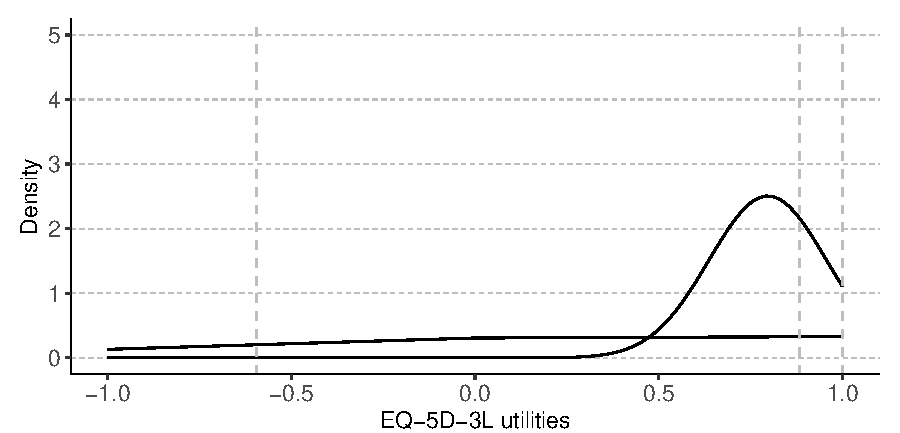
\includegraphics{aldvmm_vignette_files/figure-latex/fig-comp-dens1-1.pdf}
\caption{\label{fig:fig-comp-dens1}Densities in components based on ``Nelder-Mead'' parameter estimates (observation with population average Oxford Hip Score 3.8489)}
\end{figure}

\begin{figure}
\centering
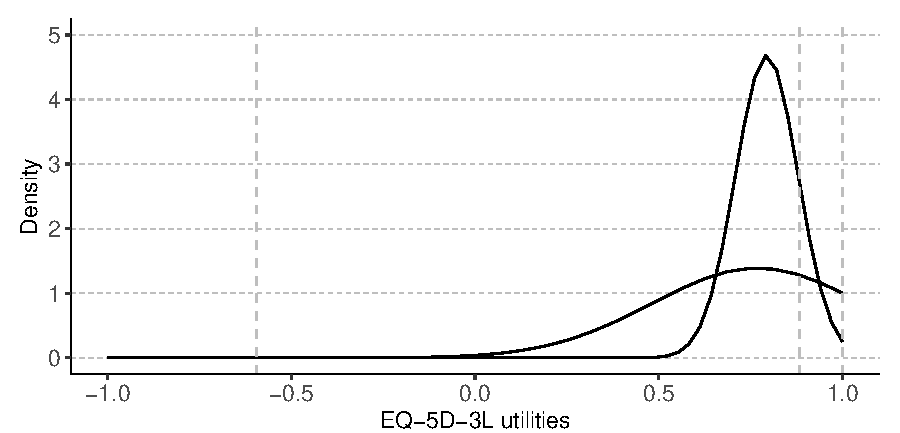
\includegraphics{aldvmm_vignette_files/figure-latex/fig-comp-dens2-1.pdf}
\caption{\label{fig:fig-comp-dens2}Densities in components based on ``nlminb'' parameter estimates (observation with population average Oxford Hip Score 3.8489)}
\end{figure}

\begin{figure}
\centering
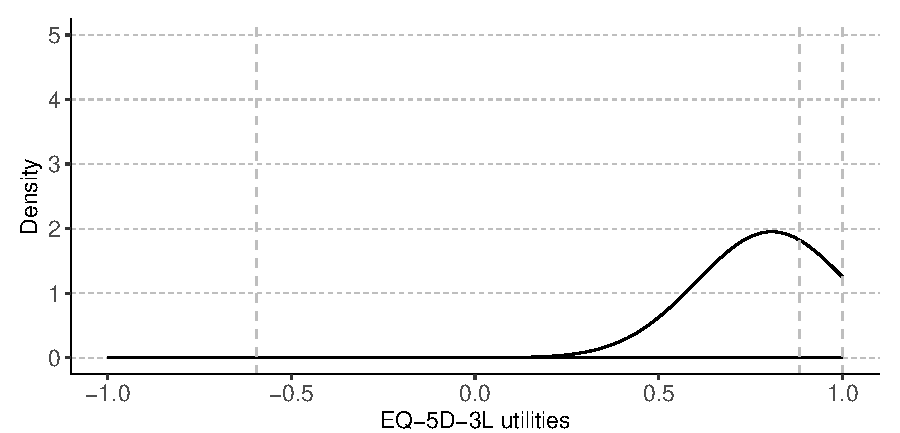
\includegraphics{aldvmm_vignette_files/figure-latex/fig-comp-dens3-1.pdf}
\caption{\label{fig:fig-comp-dens3}Densities in components based on ``hjn'' parameter estimates (observation with population average Oxford Hip Score 3.8489)}
\end{figure}

The differences in parameter estimates from different optimization methods show that the choice of the optimization algorithm and initial values is very important for parameter identification. As adjusted limited dependent variable mixture models are frequently used for tasks that rely on predictions, we also compare expected values from the ``Nelder-Mead'' and ``hjn'' methods to expected values from the ``nlminb'' method. Expected values from the ``Nelder-Mead'' and ``hjn'' methods differed from expected values from the ``nlminb'' method among observations with lower expected values (figure \ref{fig:plot-comp-pred}).

\begin{figure}
\centering
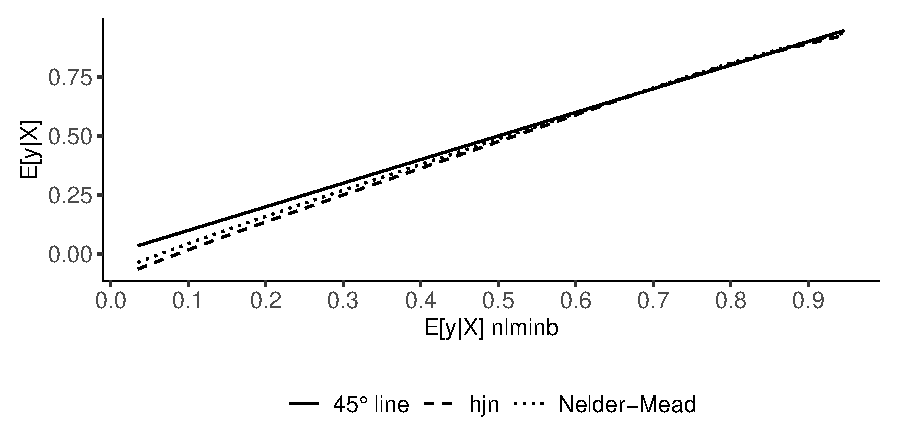
\includegraphics{aldvmm_vignette_files/figure-latex/plot-comp-pred-1.pdf}
\caption{\label{fig:plot-comp-pred}Expected values from model 1, ``Nelder-Mead'' and ``hjn'' versus ``nlminb'' with zero starting values}
\end{figure}

An visual inspection of mean residuals over deciles of expected values shows that model 1 fits the data poorly regardless of the optimization method, and that the patterns of over- and under-predictions of observed values are similar across optimization methods despite different log-likelihoods (figure \ref{fig:plot-comp-mhl1}, figure \ref{fig:plot-comp-mhl2} and figure \ref{fig:plot-comp-mhl3} in the appendix).

\hypertarget{constrained-optimization-with-user-defined-initial-values}{%
\subsubsection{Constrained optimization with user-defined initial values}\label{constrained-optimization-with-user-defined-initial-values}}

We can also fit model 1 with user-defined starting values and box constraints. When constraints are imposed, the aldvmm() function uses the optimization method ``L-BFGS-B,'' which shows very sensitive to starting values. We use zero initial values for all parameters except for the intercept in the multinomial logit which we set to the estimate from the ``nlminb'' optimization method with ``zero'' sarting values (0.7283) (table \ref{tab:tab-comp-coef}). We impose a lower limit of -3 to the log-standard deviations in both components. The aldvmm() function returns a warning that the covariance matrix included negative values on the diagonal. We see that these values are the variances of the intercept and the log-standard deviation in component 2 (table \ref{tab:tab-sum-cstr}). The log-likelihood amounts to -627.78, which is even lower than the log-likelihood in the solution of the ``Nelder-Mead'' optimization method with ``zero'' starting values. The parameter estimates do not resemble any of the solutions of the unconstrained ``Nelder-Mead,'' ``nlminb'' or ``hjn'' optimization methods with ``zero'' values (table \ref{tab:tab-comp-coef}), which further emphasizes the difficulties in finding a global optimum of the likelihood with English EQ-5D-3L utilities after hip replacement.

\begin{Shaded}
\begin{Highlighting}[]
\NormalTok{init }\OtherTok{\textless{}{-}} \FunctionTok{c}\NormalTok{(}\DecValTok{0}\NormalTok{,    }\DecValTok{0}\NormalTok{,   }\DecValTok{0}\NormalTok{,   }\DecValTok{0}\NormalTok{,    }\DecValTok{0}\NormalTok{,    }\DecValTok{0}\NormalTok{,    }\FloatTok{0.7283}\NormalTok{)}
\NormalTok{lo   }\OtherTok{\textless{}{-}} \FunctionTok{c}\NormalTok{(}\SpecialCharTok{{-}}\ConstantTok{Inf}\NormalTok{, }\SpecialCharTok{{-}}\ConstantTok{Inf}\NormalTok{, }\SpecialCharTok{{-}}\DecValTok{3}\NormalTok{,  }\SpecialCharTok{{-}}\ConstantTok{Inf}\NormalTok{, }\SpecialCharTok{{-}}\ConstantTok{Inf}\NormalTok{, }\SpecialCharTok{{-}}\DecValTok{3}\NormalTok{, }\SpecialCharTok{{-}}\ConstantTok{Inf}\NormalTok{)}
\NormalTok{hi   }\OtherTok{\textless{}{-}} \FunctionTok{c}\NormalTok{(}\ConstantTok{Inf}\NormalTok{,  }\ConstantTok{Inf}\NormalTok{,  }\ConstantTok{Inf}\NormalTok{, }\ConstantTok{Inf}\NormalTok{,  }\ConstantTok{Inf}\NormalTok{,  }\ConstantTok{Inf}\NormalTok{,  }\ConstantTok{Inf}\NormalTok{)}

\NormalTok{fit1\_cstr }\OtherTok{\textless{}{-}}\NormalTok{ aldvmm}\SpecialCharTok{::}\FunctionTok{aldvmm}\NormalTok{(eq5d }\SpecialCharTok{\textasciitilde{}}\NormalTok{ hr }\SpecialCharTok{|} \DecValTok{1}\NormalTok{,}
                            \AttributeTok{data =}\NormalTok{ df,}
                            \AttributeTok{psi =} \FunctionTok{c}\NormalTok{(}\FloatTok{0.883}\NormalTok{, }\SpecialCharTok{{-}}\FloatTok{0.594}\NormalTok{),}
                            \AttributeTok{ncmp =} \DecValTok{2}\NormalTok{,}
                            \AttributeTok{init.est =}\NormalTok{ init,}
                            \AttributeTok{init.lo =}\NormalTok{ lo,}
                            \AttributeTok{init.hi =}\NormalTok{ hi)}

\FunctionTok{summary}\NormalTok{(fit1\_cstr)}
\end{Highlighting}
\end{Shaded}

\begin{table}[ht]
\centering
\begin{tabular}{llrrrrrr}
  \hline
 &  & Estimate & Std. Err. & z & P$>$$|$z$|$ & [95\% Conf.  & Interval] \\ 
  \hline
E[y$|$X, c] &  &  &  &  &  &  &  \\ 
   \hline
Comp1 & (Intercept) & -0.092 & 0.009 & -10.805 & 0.000 & -0.109 & -0.075 \\ 
   & hr &  0.232 & 0.002 & 101.849 & 0.000 &  0.228 &  0.237 \\ 
   & lnsigma & -1.641 & 0.009 & -183.981 & 0.000 & -1.658 & -1.623 \\ 
  Comp2 & (Intercept) & 0.393 &   NaN &   NaN &   NaN &     NaN &    NaN \\ 
   & hr & 2.525 & 7.479 & 0.338 & 0.368 & -12.135 & 17.184 \\ 
   & lnsigma & -0.765 & NaN & NaN & NaN & NaN & NaN \\ 
   \hline
P[c$|$X] &  &  &  &  &  &  &  \\ 
   \hline
Comp1 & (Intercept) & 6.852 & 0.539 & 12.717 & 0.000 & 5.796 & 7.908 \\ 
   \hline
N = 10549 & ll = -627.78 & AIC = 1269.55 & BIC = 1269.55 &  &  &  &  \\ 
  \end{tabular}
\end{table}

\hypertarget{single-component-model}{%
\subsubsection{Single-component model}\label{single-component-model}}

As the solution of the ``hjn'' algorithm included a component with very low probability, we also estimate a single-component model.

\begin{Shaded}
\begin{Highlighting}[]
\NormalTok{fit }\OtherTok{\textless{}{-}}\NormalTok{ aldvmm}\SpecialCharTok{::}\FunctionTok{aldvmm}\NormalTok{(eq5d }\SpecialCharTok{\textasciitilde{}}\NormalTok{ hr,}
                      \AttributeTok{data =}\NormalTok{ df,}
                      \AttributeTok{psi =} \FunctionTok{c}\NormalTok{(}\FloatTok{0.883}\NormalTok{, }\SpecialCharTok{{-}}\FloatTok{0.594}\NormalTok{),}
                      \AttributeTok{ncmp =} \DecValTok{1}\NormalTok{,}
                      \AttributeTok{init.method =} \StringTok{"zero"}\NormalTok{,}
                      \AttributeTok{optim.method =} \StringTok{"nlminb"}\NormalTok{)}

\FunctionTok{summary}\NormalTok{(fit)}
\end{Highlighting}
\end{Shaded}

The coefficients of the single-component model are relatively similar to the parameters in the second component of model 1 from the ``hjn'' algorithm (table \ref{tab:tab-sum-tobit}). The Akaike information criterion amounts to 1'275.61 which is larger than the values of the ``nlminb'' (-1'398.65) and ``hjn'' (-66'100.87) solutions of the two-component model and thus suggests worse fit of the single-component model.\footnote{In the aldvmm() output, smaller values of the Akaike information criterion indicate better goodness of fit.}

\begin{table}[ht]
\centering
\caption{Regression results of model1 with 1 component, 
                     zero starting values in "nlminb" algorithm} 
\label{tab:tab-sum-tobit}
\begin{tabular}{llrrrrrr}
  \hline
 &  & Estimate & Std. Err. & z & P$>$$|$z$|$ & [95\% Conf.  & Interval] \\ 
  \hline
E[y$|$X, c] &  &  &  &  &  &  &  \\ 
   \hline
Comp1 & (Intercept) & -0.089 & 0.009 & -10.410 & 0.000 & -0.105 & -0.072 \\ 
   & hr &  0.232 & 0.002 & 101.468 & 0.000 &  0.227 &  0.236 \\ 
   & lnsigma & -1.636 & 0.009 & -184.242 & 0.000 & -1.654 & -1.619 \\ 
   \hline
N = 10549 & ll = -634.81 & AIC = 1275.61 & BIC = 1275.61 &  &  &  &  \\ 
  \end{tabular}
\end{table}

\hypertarget{model-2}{%
\subsection{Model 2}\label{model-2}}

As an alternative specification, we explore model 2 with a coefficient of the Oxford Hip score in the multinomial logit model of component membership. For this fit, we use the method ``nlminb'' with estimates from Hernández Alava and Wailoo (2015) as starting values.

\begin{Shaded}
\begin{Highlighting}[]
\NormalTok{init }\OtherTok{\textless{}{-}} \FunctionTok{c}\NormalTok{(}\SpecialCharTok{{-}}\NormalTok{.}\DecValTok{40293118}\NormalTok{, .}\DecValTok{30502755}\NormalTok{, .}\DecValTok{22614716}\NormalTok{, .}\DecValTok{14801581}\NormalTok{, }\SpecialCharTok{{-}}\NormalTok{.}\DecValTok{70755741}\NormalTok{, }\DecValTok{0}\NormalTok{, }
          \SpecialCharTok{{-}}\FloatTok{1.2632051}\NormalTok{, }\SpecialCharTok{{-}}\FloatTok{2.4541401}\NormalTok{)}

\NormalTok{fit2 }\OtherTok{\textless{}{-}}\NormalTok{ aldvmm}\SpecialCharTok{::}\FunctionTok{aldvmm}\NormalTok{(eq5d }\SpecialCharTok{\textasciitilde{}}\NormalTok{ hr }\SpecialCharTok{|}\NormalTok{ hr,}
                       \AttributeTok{data =}\NormalTok{ df,}
                       \AttributeTok{psi =} \FunctionTok{c}\NormalTok{(}\FloatTok{0.883}\NormalTok{, }\SpecialCharTok{{-}}\FloatTok{0.594}\NormalTok{),}
                       \AttributeTok{ncmp =} \DecValTok{2}\NormalTok{,}
                       \AttributeTok{init.est =}\NormalTok{ init,}
                       \AttributeTok{optim.method =} \StringTok{"nlminb"}\NormalTok{)}

\FunctionTok{summary}\NormalTok{(fit2)}
\end{Highlighting}
\end{Shaded}

The Akaike information criterion of model 2 fitted using the ``nlminb'' method amounts to -1'862.44 which is smaller than the Akaike information criterion of model 1 (-1'398.65) with the same method. The smaller Akaike information criterion suggests that the increase in the log-likelihood after inclusion of a coefficient of the Oxford Hip Score on the probability of component membership is sufficiently large to justify the extra parameter.\footnote{In the aldvmm() output, smaller values of the Akaike information criterion indicate better goodness of fit.}

\begin{table}[ht]
\centering
\caption{Regression results of model 2 with user-defined 
                     starting values in the "nlminb" algorithm} 
\label{tab:tab-sum-mod2}
\begin{tabular}{llrrrrrr}
  \hline
 &  & Estimate & Std. Err. & z & P$>$$|$z$|$ & [95\% Conf.  & Interval] \\ 
  \hline
E[y$|$X, c] &  &  &  &  &  &  &  \\ 
   \hline
Comp1 & (Intercept) & -0.119 & 0.015 & -7.932 & 0.000 & -0.149 & -0.090 \\ 
   & hr &  0.080 & 0.006 & 13.665 & 0.000 &  0.069 &  0.092 \\ 
   & lnsigma & -1.872 & 0.035 & -53.692 & 0.000 & -1.940 & -1.804 \\ 
  Comp2 & (Intercept) & 0.201 & 0.006 & 31.772 & 0.000 & 0.189 & 0.213 \\ 
   & hr & 0.156 & 0.002 & 94.616 & 0.000 & 0.153 & 0.159 \\ 
   & lnsigma & -2.213 & 0.011 & -202.408 & 0.000 & -2.235 & -2.192 \\ 
   \hline
P[c$|$X] &  &  &  &  &  &  &  \\ 
   \hline
Comp1 & (Intercept) &  1.774 & 0.131 &  13.534 & 0.000 &  1.517 &  2.031 \\ 
   & hr & -1.353 & 0.044 & -30.574 & 0.000 & -1.439 & -1.266 \\ 
   \hline
N = 10549 & ll = 939.22 & AIC = -1862.44 & BIC = -1862.44 &  &  &  &  \\ 
  \end{tabular}
\end{table}

\hypertarget{comparison-to-stata-results}{%
\subsection{\texorpdfstring{Comparison to STATA\textsuperscript{\textregistered} results}{Comparison to STATA results}}\label{comparison-to-stata-results}}

To validate the R implementation of adjusted limited dependent variable mixture models, we estimate the four models presented in Hernández Alava and Wailoo (2015) as reference cases in R and STATA\textsuperscript{\textregistered}.\footnote{The STATA\textsuperscript{\textregistered} and R code for model estimation is included in the appendix.}

\begin{enumerate}
\def\labelenumi{\arabic{enumi}.}
\item
  Model 1 with default options
\item
  Model 1 with parameter constraints
\item
  Model 1 with initial values from constant-only model
\item
  Model 2 with user-defined initial values
\end{enumerate}

The parameter estimates and standard errors obtained in R are very similar to the results from STATA\textsuperscript{\textregistered} (table \ref{tab:tab-comp-stata} and table \ref{tab:tab-compse-stata}). R did not obtain any standard errors in reference model 2 while STATA\textsuperscript{\textregistered} returned standard errors for the first component and the probability of belonging to component 1. Although reference models 1 and 3 yield different parameter estimates, they converged at the same log-likelihood which further supports the hypothesis of multiple local optima of the likelihood. The log-likelihood is consistently smaller in R than in STATA\textsuperscript{\textregistered}, but the relative ordering of models is consistent across platforms.

\begin{table}[ht]
\centering
\caption{Comparison of point estimates to the results of the STATA package} 
\label{tab:tab-comp-stata}
\begin{tabular}{llrrrrrrrr}
  \hline
  &  & (1) &  & (2) &  & (3) &  & (4) &  \\ 
   &  & R & STATA & R & STATA & R & STATA & R & STATA \\ 
   \hline
E[y$|$X, c] &  &  &  &  &  &  &  &  &  \\ 
   \hline
Comp1 & (Intercept) & -0.431 & -0.427 & -0.092 & -0.092 & 0.236 & 0.236 & 0.003 & 0.006 \\ 
   & hr &  0.313 & 0.312 &  0.232 & 0.232 & 0.146 & 0.146 & 0.097 & 0.095 \\ 
   & lnsigma & -1.248 & -1.251 & -1.641 & -1.641 & -2.462 & -2.463 & -1.268 & -1.274 \\ 
  Comp2 & (Intercept) & 0.236 & 0.236 & 100.000 & 100.000 & -0.431 & -0.427 & 0.182 & 0.182 \\ 
   & hr & 0.146 & 0.146 &   0.000 & 0.000 &  0.313 & 0.312 & 0.161 & 0.161 \\ 
   & lnsigma & -2.462 & -2.463 & 0.000 & 0.000 & -1.248 & -1.251 & -2.281 & -2.280 \\ 
   \hline
P[c$|$X] &  &  &  &  &  &  &  &  &  \\ 
   \hline
Comp1 & (Intercept) & -0.728 & -0.725 & 6.856 & 6.855 & 0.728 & 0.725 &  2.445 & 2.448 \\ 
   & hr &  &  &  &  &  &  & -1.390 & -1.393 \\ 
   \hline
N = 10549 & ll & 706.32 & 715.84 & -627.78 & -613.7 & 706.32 & 715.84 & 941.36 & 953.2 \\ 
  \end{tabular}
\end{table}
\begin{table}[!ht]
\centering
\caption{Comparison of standard errors to the results of the STATA package.} 
\label{tab:tab-compse-stata}
\begin{tabular}{llrrrrrrrr}
  \hline
  &  & (1) &  & (2) &  & (3) &  & (4) &  \\ 
   &  & R & STATA & R & STATA & R & STATA & R & STATA \\ 
   \hline
E[y$|$X, c] &  &  &  &  &  &  &  &  &  \\ 
   \hline
Comp1 & (Intercept) & 0.022 & 0.022 & NA & 0.009 & 0.007 & 0.007 & 0.028 & 0.028 \\ 
   & hr & 0.007 & 0.006 & NA & 0.002 & 0.002 & 0.002 & 0.012 & 0.012 \\ 
   & lnsigma & 0.022 & 0.021 & NA & 0.009 & 0.018 & -0.018 & 0.031 & 0.032 \\ 
  Comp2 & (Intercept) & 0.007 & 0.007 & NA &  & 0.022 & 0.022 & 0.007 & 0.007 \\ 
   & hr & 0.002 & 0.002 & NA &  & 0.007 & 0.006 & 0.002 & 0.002 \\ 
   & lnsigma & 0.018 & 0.018 & NA &  & 0.022 & 0.021 & 0.013 & 0.013 \\ 
   \hline
P[c$|$X] &  &  &  &  &  &  &  &  &  \\ 
   \hline
Comp1 & (Intercept) & 0.061 & 0.061 & NA & 0.540 & 0.061 & 0.061 & 0.172 & 0.172 \\ 
   & hr &  &  &  &  &  &  & 0.057 & 0.056 \\ 
   \hline
N = 10549 & ll & 706.32 & 715.84 & -627.78 & -613.7 & 706.32 & 715.84 & 941.36 & 953.2 \\ 
  \end{tabular}
\end{table}

Fitted values show very similar marginal distributions on both platforms (figure \ref{fig:box-pred-yhat-stata}). R does not return fitted values in reference case 2. The summary statistics of differences in fitted values between R and STATA\textsuperscript{\textregistered} suggest that individual predictions are quite similar across platforms as well (table \ref{tab:compyhat}.

Standard errors of fitted values differ visibly between platforms (figure \ref{fig:box-pred-se-stata} and table \ref{tab:compse}). The difference is particularly pronounced in reference case 1, but the standard errors from STATA\textsuperscript{\textregistered} seem quite extreme compared to all other reference cases. R does not return standard errors of fitted values in reference case 2.

\begin{figure}
\centering
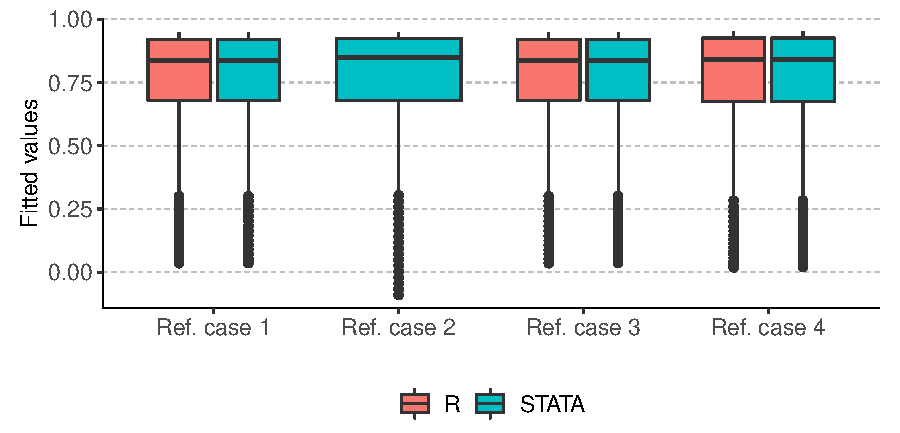
\includegraphics{aldvmm_vignette_files/figure-latex/box-pred-yhat-stata-1.pdf}
\caption{\label{fig:box-pred-yhat-stata}Fitted values in R and STATA}
\end{figure}

\begin{figure}
\centering
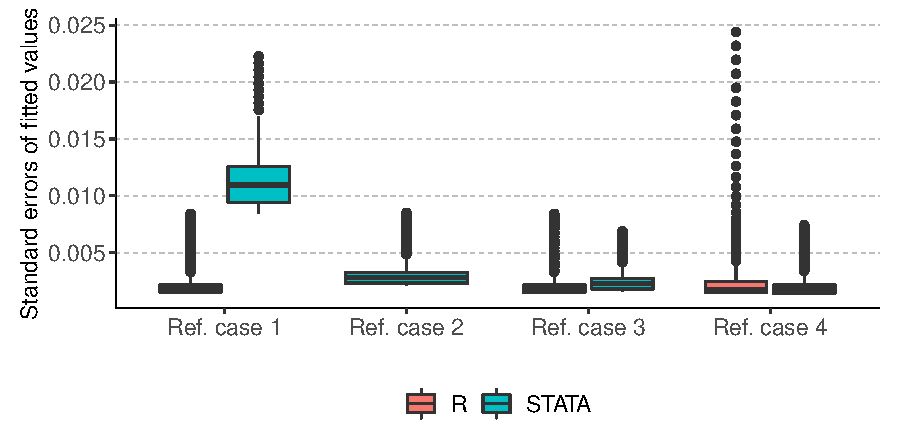
\includegraphics{aldvmm_vignette_files/figure-latex/box-pred-se-stata-1.pdf}
\caption{\label{fig:box-pred-se-stata}Standard errors of fitted values in R and STATA}
\end{figure}

\begin{table}[ht]
\centering
\caption{Summary statistics of differences of fitted values in R and STATA (positive values suggest larger values in STATA)} 
\label{tab:compyhat}
\begin{tabular}{lrrrr}
  \hline
 & Ref. case 1 & Ref. case 2 & Ref. case 3 & Ref. case 4 \\ 
  \hline
Min. & -0.000038 &  & -0.000038 & -0.000051 \\ 
  1st Qu. & -0.000036 &  & -0.000036 & -0.000044 \\ 
  Median & -0.000033 &  & -0.000033 & 0.000008 \\ 
  Mean & 0.000037 &  & 0.000037 & 0.000035 \\ 
  3rd Qu. & 0.000047 &  & 0.000047 & 0.000070 \\ 
  Max. & 0.000567 &  & 0.000567 & 0.002319 \\ 
   \hline
\end{tabular}
\end{table}

\begin{table}[ht]
\centering
\caption{Summary statistics of differences of standard errors of fitted values in R and STATA (positive values suggest larger values in STATA)} 
\label{tab:compse}
\begin{tabular}{lrrrr}
  \hline
 & Ref. case 1 & Ref. case 2 & Ref. case 3 & Ref. case 4 \\ 
  \hline
Min. & 0.005897 &  & -0.002063 & -0.016984 \\ 
  1st Qu. & 0.006898 &  & -0.000551 & -0.000823 \\ 
  Median & 0.008690 &  & 0.000189 & -0.000364 \\ 
  Mean & 0.008917 &  & 0.000171 & -0.000515 \\ 
  3rd Qu. & 0.011050 &  & 0.001054 & 0.000354 \\ 
  Max. & 0.013830 &  & 0.001530 & 0.000792 \\ 
   \hline
\end{tabular}
\end{table}

The comparison of the R and STATA\textsuperscript{\textregistered} packages showed that the R implementation sometimes behaves differently than the STATA\textsuperscript{\textregistered} package, but the results are not indicative of technical errors in the R implementation.

\hypertarget{discussion}{%
\section{Discussion}\label{discussion}}

Adjusted limited dependent variable mixture models are powerful tools for regression analysis of health state utilities. Unlike standard regression models, adjusted limited dependent variable mixture models account for limits, gaps and multi-modal distributions.

The comparison of different optimization methods with EQ-5D-3L utility data from English patients after hip replacement in 2011 and 2012 (NHS Digital 2013) shows that the likelihood function can be challenging to maximize and can converge at extreme solutions. Parameter estimates vary considerably across optimization methods and even across methods with the same maximum log-likelihood. However, fitted values are very similar across the four reference cases which suggests that the model is more robust for the identification of incremental and average marginal effects than for parameter identification.

The `aldvmm' package offers a variety of optimization algorithms and methods for generating initial values which is an important strength in such challenging situations. It is essential to assess different optimization algorithms and methods for initial values before interpreting the parameter estimates or predictions of adjusted limited dependent variable mixture models.

The analysis of the EQ-5D-3L utility data also suggests that simpler models with fewer components should be considered when multi-component models are difficult to fit. Even single-component adjusted limited dependent variable mixture models can improve fit compared to traditional regression techniques because they account for limits and gaps.

Although coefficients can be interpreted as marginal effects within each component, they cannot interpreted in terms of overall expected values. Thus, average marginal effects and average treatment effects need to be calculated from predictions using the generic function predict(). Standard errors of marginal effects or average treatment effects can be calculated using the standard errors of fitted values for observed and counterfactual covariate values.

In situations with repeated utility measures, the `aldvmm' package only allows fixed effects estimations with individual/group and time fixed effects which can be an important limitation in the analysis of clinical data. However, time fixed effects can be an appropriate modeling strategy in the presence of general time trends and dynamic selection in the population, e.g.~because health state utilities decrease over time and treated individuals survive longer and thus are over-represented in later measurements. In light of the trade-off between the efficiency of the random effects model and the causal interpretation of treatment effects in a fixed-effects model it is recommended to assess the uncorrelatedness of random effects with the treatment using the Hausman test in a generalized linear model.

Possible extensions of `aldvmm' could include adjusted limited dependent variable beta mixture models (Gray and Alava 2018), a mixed model implementation for repeated measures and a method for the calculation of average marginal effects and their standard errors.

\newpage

\hypertarget{references}{%
\section{References}\label{references}}

\hypertarget{refs}{}
\begin{CSLReferences}{1}{0}
\leavevmode\vadjust pre{\hypertarget{ref-Dixon2020}{}}%
Dixon, Padraig, William Hollingworth, and John Sparrow. 2020. {``Mapping to Quality of Life and Capability Measures in Cataract Surgery Patients: From Cat-Prom5 to EQ-5d-3l, EQ-5d-5l, and ICECAP-o Using Mixture Modelling.''} \emph{MDM Policy \& Practice} 5 (1): 2381468320915447.

\leavevmode\vadjust pre{\hypertarget{ref-Dolan1997}{}}%
Dolan, Paul. 1997. {``Modeling Valuations for EuroQol Health States.''} \emph{Medical Care}, 1095--1108.

\leavevmode\vadjust pre{\hypertarget{ref-Dowd2014}{}}%
Dowd, Bryan E, William H Greene, and Edward C Norton. 2014. {``Computation of Standard Errors.''} \emph{Health Services Research} 49 (2): 731--50.

\leavevmode\vadjust pre{\hypertarget{ref-Fuller2017}{}}%
Fuller, Gordon Ward, Monica Hernandez, David Pallot, Fiona Lecky, Mathew Stevenson, and Belinda Gabbe. 2017. {``Health State Preference Weights for the Glasgow Outcome Scale Following Traumatic Brain Injury: A Systematic Review and Mapping Study.''} \emph{Value in Health} 20 (1): 141--51.

\leavevmode\vadjust pre{\hypertarget{ref-Gray2018b}{}}%
Gray, Laura A, and Mónica Hernández Alava. 2018. {``A Command for Fitting Mixture Regression Models for Bounded Dependent Variables Using the Beta Distribution.''} \emph{The Stata Journal} 18 (1): 51--75.

\leavevmode\vadjust pre{\hypertarget{ref-Gray2018}{}}%
Gray, Laura A, Mónica Hernández Alava, and Allan J Wailoo. 2018. {``Development of Methods for the Mapping of Utilities Using Mixture Models: Mapping the AQLQ-s to the EQ-5d-5l and the Hui3 in Patients with Asthma.''} \emph{Value in Health} 21 (6): 748--57.

\leavevmode\vadjust pre{\hypertarget{ref-Gray2018a}{}}%
Gray, Laura A, Allan J Wailoo, and Monica Hernandez Alava. 2018. {``Mapping the FACT-b Instrument to EQ-5d-3l in Patients with Breast Cancer Using Adjusted Limited Dependent Variable Mixture Models Versus Response Mapping.''} \emph{Value in Health} 21 (12): 1399--1405.

\leavevmode\vadjust pre{\hypertarget{ref-HernandezAlava2015}{}}%
Hernández Alava, Mónica, and Allan Wailoo. 2015. {``Fitting Adjusted Limited Dependent Variable Mixture Models to {EQ-5d}.''} \emph{The Stata Journal} 15 (3): 737--50.

\leavevmode\vadjust pre{\hypertarget{ref-HernandezAlava2012}{}}%
Hernández Alava, Mónica, Allan J Wailoo, and Roberta Ara. 2012. {``Tails from the Peak District: Adjusted Limited Dependent Variable Mixture Models of {EQ-5d} Questionnaire Health State Utility Values.''} \emph{Value in Health} 15 (3): 550--61.

\leavevmode\vadjust pre{\hypertarget{ref-HernandezAlava2013}{}}%
Hernández Alava, Mónica, Allan Wailoo, Fred Wolfe, and Kaleb Michaud. 2013. {``The Relationship Between {EQ-5d}, {HAQ} and Pain in Patients with Rheumatoid Arthritis.''} \emph{Rheumatology} 52 (5): 944--50.

\leavevmode\vadjust pre{\hypertarget{ref-HernandezAlava2014}{}}%
---------. 2014. {``A Comparison of Direct and Indirect Methods for the Estimation of Health Utilities from Clinical Outcomes.''} \emph{Medical Decision Making} 34 (7): 919--30.

\leavevmode\vadjust pre{\hypertarget{ref-Hvidberg2016}{}}%
Hvidberg, Michael Falk. 2016. {``A Framework for Identifying Disease Burden and Estimating Health-Related Quality of Life and Prevalence Rates for 199 Medically Defined Chronic Conditions.''}

\leavevmode\vadjust pre{\hypertarget{ref-Mukuria2019}{}}%
Mukuria, Clara, Donna Rowen, Sue Harnan, Andrew Rawdin, Ruth Wong, Roberta Ara, and John Brazier. 2019. {``An Updated Systematic Review of Studies Mapping (or Cross-Walking) Measures of Health-Related Quality of Life to Generic Preference-Based Measures to Generate Utility Values.''} \emph{Applied Health Economics and Health Policy}, 1--19.

\leavevmode\vadjust pre{\hypertarget{ref-Mulhern2018}{}}%
Mulhern, Brendan, Yan Feng, Koonal Shah, Mathieu F Janssen, Michael Herdman, Ben van Hout, and Nancy Devlin. 2018. {``Comparing the UK EQ-5d-3l and English EQ-5d-5l Value Sets.''} \emph{Pharmacoeconomics} 36 (6): 699--713.

\leavevmode\vadjust pre{\hypertarget{ref-NHSDigital2013}{}}%
NHS Digital. 2013. {``Finalised Patient Reported Outcome Measures (PROMs) in England - April 2011 to March 2012. Patient Reported Outcome Measures (PROMs).''} \emph{Https://Digital.nhs.uk/Data-and-Information/Publications/Statistical/Patient-Reported-Outcome-Measures-Proms/Finalised-Patient-Reported-Outcome-Measures-Proms-in-England-April-2011-to-March-2012} October 15, 2013.

\leavevmode\vadjust pre{\hypertarget{ref-Pennington2020}{}}%
Pennington, Becky M, Mónica Hernández-Alava, Philip Hykin, Sobha Sivaprasad, Laura Flight, Abualbishr Alshreef, and John Brazier. 2020. {``Mapping from Visual Acuity to EQ-5d, EQ-5d with Vision Bolt-on, and VFQ-UI in Patients with Macular Edema in the LEAVO Trial.''} \emph{Value in Health} 23 (7): 928--35.

\leavevmode\vadjust pre{\hypertarget{ref-Whitmore1986}{}}%
Whitmore, GA. 1986. {``Prediction Limits for a Univariate Normal Observation.''} \emph{The American Statistician} 40 (2): 141--43.

\leavevmode\vadjust pre{\hypertarget{ref-Xu2020}{}}%
Xu, Richard Huan, Eliza Lai Yi Wong, Jun Jin, Ying Dou, and Dong Dong. 2020. {``Mapping of the EORTC QLQ-C30 to EQ-5d-5l Index in Patients with Lymphomas.''} \emph{The European Journal of Health Economics} 21 (9): 1363--73.

\leavevmode\vadjust pre{\hypertarget{ref-Yang2019}{}}%
Yang, Fan, Carlos KH Wong, Nan Luo, James Piercy, Rebecca Moon, and James Jackson. 2019. {``Mapping the Kidney Disease Quality of Life 36-Item Short Form Survey (KDQOL-36) to the EQ-5d-3l and the EQ-5d-5l in Patients Undergoing Dialysis.''} \emph{The European Journal of Health Economics} 20 (8): 1195--1206.

\end{CSLReferences}

\newpage

\hypertarget{appendix}{%
\section{Appendix}\label{appendix}}

\hypertarget{covariance-matrices-across-optimization-methods}{%
\subsection{Covariance matrices across optimization methods}\label{covariance-matrices-across-optimization-methods}}

Covariance matrices were incomplete or missing entirely (\texttt{FALSE}) in multiple optimization approaches (table \ref{tab:cov})

\begin{table}[ht]
\centering
\caption{Covariance matrix by optimization method} 
\label{tab:cov}
\begin{tabular}{lrrrrrrrr}
  \hline
 & Nelder-Mead & BFGS & CG & L-BFGS-B & nlminb & Rcgmin & Rvmmin & hjn \\ 
  \hline
zero & FALSE & TRUE & TRUE & FALSE & TRUE & TRUE & TRUE & TRUE \\ 
  random & FALSE & TRUE & FALSE & FALSE & TRUE & TRUE & FALSE & FALSE \\ 
  constant & FALSE & TRUE & FALSE & FALSE & TRUE & TRUE & FALSE & TRUE \\ 
  sann & TRUE & TRUE & TRUE & TRUE & TRUE & TRUE & TRUE & TRUE \\ 
   \hline
\end{tabular}
\end{table}

\newpage

\hypertarget{modified-hosmer-lemeshow-test}{%
\subsection{Modified Hosmer-Lemeshow test}\label{modified-hosmer-lemeshow-test}}

\begin{Shaded}
\begin{Highlighting}[]
\CommentTok{\# Number of percentiles  }
\NormalTok{ngroup }\OtherTok{\textless{}{-}} \DecValTok{10}

\CommentTok{\# Extract expected values and residuals}
\NormalTok{yhat }\OtherTok{\textless{}{-}}\NormalTok{ fit1\_all[[}\StringTok{"zero"}\NormalTok{]][[}\StringTok{"Nelder{-}Mead"}\NormalTok{]][[}\StringTok{"pred"}\NormalTok{]][[}\StringTok{"yhat"}\NormalTok{]]}
\NormalTok{res }\OtherTok{\textless{}{-}}\NormalTok{ fit1\_all[[}\StringTok{"zero"}\NormalTok{]][[}\StringTok{"Nelder{-}Mead"}\NormalTok{]][[}\StringTok{"pred"}\NormalTok{]][[}\StringTok{"res"}\NormalTok{]]}

\CommentTok{\# Make groups}
\NormalTok{group }\OtherTok{\textless{}{-}} \FunctionTok{as.numeric}\NormalTok{(}\FunctionTok{cut}\NormalTok{(yhat, }\AttributeTok{breaks =}\NormalTok{ ngroup), }\AttributeTok{na.rm=}\ConstantTok{TRUE}\NormalTok{)}

\CommentTok{\# Auxiliary regression}
\NormalTok{aux }\OtherTok{\textless{}{-}}\NormalTok{ stats}\SpecialCharTok{::}\FunctionTok{lm}\NormalTok{(res }\SpecialCharTok{\textasciitilde{}} \FunctionTok{factor}\NormalTok{(group))}

\CommentTok{\# Data set of predictions from auxiliary regressions}
\NormalTok{newdf }\OtherTok{\textless{}{-}} \FunctionTok{data.frame}\NormalTok{(}\AttributeTok{group =} \FunctionTok{unique}\NormalTok{(group)[}\FunctionTok{order}\NormalTok{(}\FunctionTok{unique}\NormalTok{(group))])}
\NormalTok{predict }\OtherTok{\textless{}{-}} \FunctionTok{predict}\NormalTok{(aux, }
                   \AttributeTok{newdata =}\NormalTok{ newdf, }
                   \AttributeTok{se.fit =} \ConstantTok{TRUE}\NormalTok{, }
                   \AttributeTok{interval =} \StringTok{\textquotesingle{}confidence\textquotesingle{}}\NormalTok{, }
                   \AttributeTok{level =} \FloatTok{0.95}\NormalTok{)}

\NormalTok{plotdat }\OtherTok{\textless{}{-}} \FunctionTok{as.data.frame}\NormalTok{(}\FunctionTok{rbind}\NormalTok{(}
  \FunctionTok{cbind}\NormalTok{(}\AttributeTok{group =}\NormalTok{ newdf}\SpecialCharTok{$}\NormalTok{group, }
        \AttributeTok{outcome =} \StringTok{"mean"}\NormalTok{,}
        \AttributeTok{value =}\NormalTok{ predict}\SpecialCharTok{$}\NormalTok{fit[ , }\StringTok{\textquotesingle{}fit\textquotesingle{}}\NormalTok{]),}
  \FunctionTok{cbind}\NormalTok{(}\AttributeTok{group =}\NormalTok{ newdf}\SpecialCharTok{$}\NormalTok{group, }
        \AttributeTok{outcome =} \StringTok{"ll"}\NormalTok{,}
        \AttributeTok{value =}\NormalTok{ predict}\SpecialCharTok{$}\NormalTok{fit[ , }\StringTok{\textquotesingle{}lwr\textquotesingle{}}\NormalTok{]),}
  \FunctionTok{cbind}\NormalTok{(}\AttributeTok{group =}\NormalTok{ newdf}\SpecialCharTok{$}\NormalTok{group, }
        \AttributeTok{outcome =} \StringTok{"ul"}\NormalTok{,}
        \AttributeTok{value =}\NormalTok{ predict}\SpecialCharTok{$}\NormalTok{fit[ , }\StringTok{\textquotesingle{}upr\textquotesingle{}}\NormalTok{])}
\NormalTok{))}

\CommentTok{\# Make plot}
\NormalTok{plot }\OtherTok{\textless{}{-}}\NormalTok{ ggplot2}\SpecialCharTok{::}\FunctionTok{ggplot}\NormalTok{(plotdat, }\FunctionTok{aes}\NormalTok{(}\AttributeTok{x =} \FunctionTok{factor}\NormalTok{(}\FunctionTok{as.numeric}\NormalTok{(group)), }
                                     \AttributeTok{y =} \FunctionTok{as.numeric}\NormalTok{(value), }
                                     \AttributeTok{group =} \FunctionTok{factor}\NormalTok{(outcome))) }\SpecialCharTok{+}
  \FunctionTok{geom\_line}\NormalTok{(}\FunctionTok{aes}\NormalTok{(}\AttributeTok{linetype =} \FunctionTok{factor}\NormalTok{(outcome)))}
\end{Highlighting}
\end{Shaded}

\begin{figure}
\centering
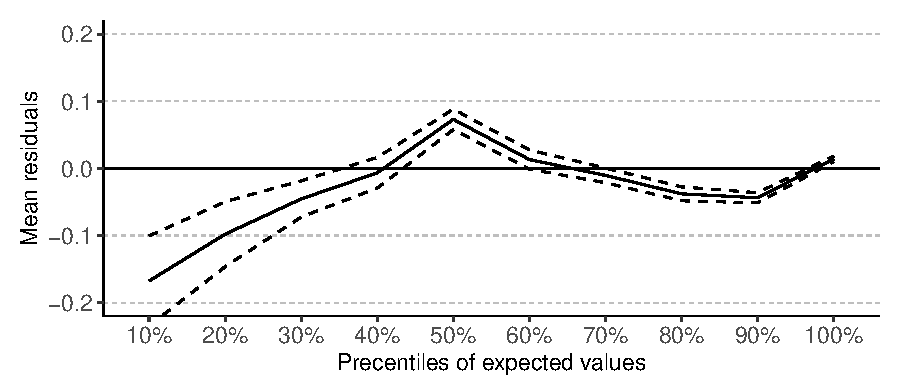
\includegraphics{aldvmm_vignette_files/figure-latex/plot-comp-mhl1-1.pdf}
\caption{\label{fig:plot-comp-mhl1}Mean residuals over deciles of expected values, ``Nelder-Mead'' with ``zero'' starting values}
\end{figure}

\begin{figure}
\centering
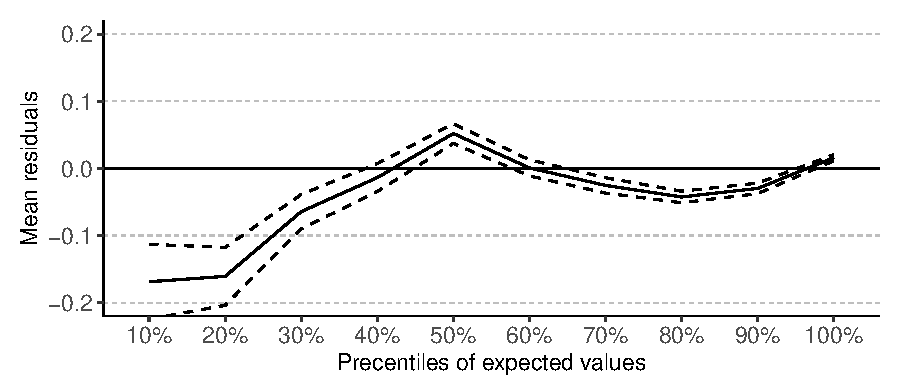
\includegraphics{aldvmm_vignette_files/figure-latex/plot-comp-mhl2-1.pdf}
\caption{\label{fig:plot-comp-mhl2}Mean residuals over deciles of expected values, ``BFGS'' with ``zero'' starting values}
\end{figure}

\begin{figure}
\centering
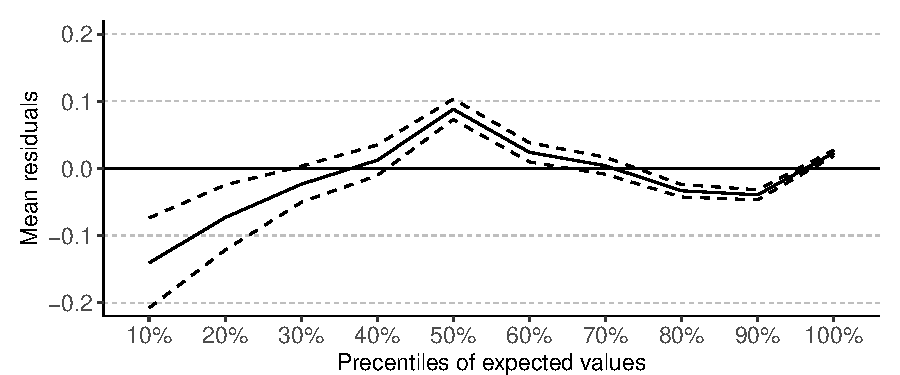
\includegraphics{aldvmm_vignette_files/figure-latex/plot-comp-mhl3-1.pdf}
\caption{\label{fig:plot-comp-mhl3}Mean residuals over deciles of expected values, ``hjn'' with ``zero'' starting values}
\end{figure}

\newpage

\hypertarget{r-code-for-the-estimation-of-reference-cases}{%
\subsection{R code for the estimation of reference cases}\label{r-code-for-the-estimation-of-reference-cases}}

\begin{Shaded}
\begin{Highlighting}[]
\CommentTok{\# (1) Reference case 1 with default optimization settings}
\NormalTok{fit1\_default }\OtherTok{\textless{}{-}}\NormalTok{ aldvmm}\SpecialCharTok{::}\FunctionTok{aldvmm}\NormalTok{(eq5d }\SpecialCharTok{\textasciitilde{}}\NormalTok{ hr }\SpecialCharTok{|} \DecValTok{1}\NormalTok{,}
                               \AttributeTok{data =}\NormalTok{ df,}
                               \AttributeTok{psi =} \FunctionTok{c}\NormalTok{(}\FloatTok{0.883}\NormalTok{, }\SpecialCharTok{{-}}\FloatTok{0.594}\NormalTok{),}
                               \AttributeTok{ncmp =} \DecValTok{2}\NormalTok{,}
                               \AttributeTok{init.method =} \StringTok{"zero"}\NormalTok{,}
                               \AttributeTok{optim.method =} \StringTok{"nlminb"}\NormalTok{)}

\CommentTok{\# (2) Reference case 1 with user{-}defined initial values and constraints on parameters}
\NormalTok{init }\OtherTok{\textless{}{-}} \FunctionTok{c}\NormalTok{(}\DecValTok{0}\NormalTok{,    }\DecValTok{0}\NormalTok{,   }\DecValTok{0}\NormalTok{,   }\DecValTok{0}\NormalTok{,    }\DecValTok{0}\NormalTok{,    }\DecValTok{0}\NormalTok{,    }\FloatTok{0.7283}\NormalTok{)}
\NormalTok{lo   }\OtherTok{\textless{}{-}} \FunctionTok{c}\NormalTok{(}\SpecialCharTok{{-}}\ConstantTok{Inf}\NormalTok{, }\SpecialCharTok{{-}}\ConstantTok{Inf}\NormalTok{, }\SpecialCharTok{{-}}\DecValTok{3}\NormalTok{,  }\SpecialCharTok{{-}}\ConstantTok{Inf}\NormalTok{, }\SpecialCharTok{{-}}\ConstantTok{Inf}\NormalTok{, }\SpecialCharTok{{-}}\DecValTok{3}\NormalTok{, }\SpecialCharTok{{-}}\ConstantTok{Inf}\NormalTok{)}
\NormalTok{hi   }\OtherTok{\textless{}{-}} \FunctionTok{c}\NormalTok{(}\ConstantTok{Inf}\NormalTok{,  }\ConstantTok{Inf}\NormalTok{,  }\ConstantTok{Inf}\NormalTok{, }\ConstantTok{Inf}\NormalTok{,  }\ConstantTok{Inf}\NormalTok{,  }\ConstantTok{Inf}\NormalTok{,  }\ConstantTok{Inf}\NormalTok{)}

\NormalTok{fit1\_cstr }\OtherTok{\textless{}{-}}\NormalTok{ aldvmm}\SpecialCharTok{::}\FunctionTok{aldvmm}\NormalTok{(eq5d }\SpecialCharTok{\textasciitilde{}}\NormalTok{ hr }\SpecialCharTok{|} \DecValTok{1}\NormalTok{,}
                            \AttributeTok{data =}\NormalTok{ df,}
                            \AttributeTok{psi =} \FunctionTok{c}\NormalTok{(}\FloatTok{0.883}\NormalTok{, }\SpecialCharTok{{-}}\FloatTok{0.594}\NormalTok{),}
                            \AttributeTok{ncmp =} \DecValTok{2}\NormalTok{,}
                            \AttributeTok{init.est =}\NormalTok{ init,}
                            \AttributeTok{init.lo =}\NormalTok{ lo,}
                            \AttributeTok{init.hi =}\NormalTok{ hi)}

\CommentTok{\# (3) Reference case 1 with initial values from constant{-}only model}
\NormalTok{fit1\_const }\OtherTok{\textless{}{-}}\NormalTok{ aldvmm}\SpecialCharTok{::}\FunctionTok{aldvmm}\NormalTok{(eq5d }\SpecialCharTok{\textasciitilde{}}\NormalTok{ hr }\SpecialCharTok{|} \DecValTok{1}\NormalTok{,}
                             \AttributeTok{data =}\NormalTok{ df,}
                             \AttributeTok{psi =} \FunctionTok{c}\NormalTok{(}\FloatTok{0.883}\NormalTok{, }\SpecialCharTok{{-}}\FloatTok{0.594}\NormalTok{),}
                             \AttributeTok{ncmp =} \DecValTok{2}\NormalTok{,}
                             \AttributeTok{init.method =} \StringTok{"constant"}\NormalTok{,}
                             \AttributeTok{optim.method =} \StringTok{"nlminb"}\NormalTok{)}

\CommentTok{\# (4) Reference case 2 with user{-}defined initial values.}
\NormalTok{init }\OtherTok{\textless{}{-}} \FunctionTok{c}\NormalTok{(}\SpecialCharTok{{-}}\NormalTok{.}\DecValTok{40293118}\NormalTok{, .}\DecValTok{30502755}\NormalTok{, .}\DecValTok{22614716}\NormalTok{, .}\DecValTok{14801581}\NormalTok{, }\SpecialCharTok{{-}}\NormalTok{.}\DecValTok{70755741}\NormalTok{, }\DecValTok{0}\NormalTok{, }
          \SpecialCharTok{{-}}\FloatTok{1.2632051}\NormalTok{, }\SpecialCharTok{{-}}\FloatTok{2.4541401}\NormalTok{)}

\NormalTok{fit2 }\OtherTok{\textless{}{-}}\NormalTok{ aldvmm}\SpecialCharTok{::}\FunctionTok{aldvmm}\NormalTok{(eq5d }\SpecialCharTok{\textasciitilde{}}\NormalTok{ hr }\SpecialCharTok{|}\NormalTok{ hr,}
                       \AttributeTok{data =}\NormalTok{ df,}
                       \AttributeTok{psi =} \FunctionTok{c}\NormalTok{(}\FloatTok{0.883}\NormalTok{, }\SpecialCharTok{{-}}\FloatTok{0.594}\NormalTok{),}
                       \AttributeTok{ncmp =} \DecValTok{2}\NormalTok{,}
                       \AttributeTok{init.est =}\NormalTok{ init,}
                       \AttributeTok{optim.method =} \StringTok{"nlminb"}\NormalTok{)}
\end{Highlighting}
\end{Shaded}

\newpage

\hypertarget{stata-code-for-the-estimation-of-reference-cases}{%
\subsection{\texorpdfstring{STATA\textsuperscript{\textregistered} code for the estimation of reference cases}{STATA code for the estimation of reference cases}}\label{stata-code-for-the-estimation-of-reference-cases}}

\begin{Shaded}
\begin{Highlighting}[]
\SpecialCharTok{*}\NormalTok{ (}\DecValTok{1}\NormalTok{) Reference case }\DecValTok{1}
\NormalTok{aldvmm eq5d hr, }\FunctionTok{ncomponents}\NormalTok{(}\DecValTok{2}\NormalTok{)}

\SpecialCharTok{*}\NormalTok{ (}\DecValTok{2}\NormalTok{) Reference case }\DecValTok{1}\NormalTok{ with constraints}
\NormalTok{matrix  input a }\OtherTok{=}\NormalTok{ (}\DecValTok{0}\NormalTok{, }\DecValTok{0}\NormalTok{, }\DecValTok{0}\NormalTok{, }\DecValTok{0}\NormalTok{, }\DecValTok{0}\NormalTok{, }\DecValTok{0}\NormalTok{, }\FloatTok{0.7283}\NormalTok{)}
\NormalTok{constraint }\DecValTok{1}\NormalTok{ [Comp\_2]}\SpecialCharTok{:}\NormalTok{hr10 }\OtherTok{=} \DecValTok{0}
\NormalTok{constraint }\DecValTok{2}\NormalTok{ [Comp\_2]}\SpecialCharTok{:}\NormalTok{\_cons }\OtherTok{=} \DecValTok{100}
\NormalTok{constraint }\DecValTok{3}\NormalTok{ [lns\_2]}\SpecialCharTok{:}\NormalTok{\_cons }\OtherTok{=} \FloatTok{1e{-}30}
\NormalTok{aldvmm eq5d hr, }\FunctionTok{ncomp}\NormalTok{(}\DecValTok{2}\NormalTok{) }\FunctionTok{from}\NormalTok{(a) }\FunctionTok{c}\NormalTok{(}\DecValTok{1} \DecValTok{2} \DecValTok{3}\NormalTok{)}

\SpecialCharTok{*}\NormalTok{ (}\DecValTok{3}\NormalTok{) Reference case }\DecValTok{1}\NormalTok{ initital values from constant}\SpecialCharTok{{-}}\NormalTok{only model}
\NormalTok{aldvmm eq5d hr, }\FunctionTok{ncomp}\NormalTok{(}\DecValTok{2}\NormalTok{) }\FunctionTok{inim}\NormalTok{(cons)}

\SpecialCharTok{*}\NormalTok{ (}\DecValTok{4}\NormalTok{) Reference case }\DecValTok{2}\NormalTok{ user}\SpecialCharTok{{-}}\NormalTok{defined initial values}
\NormalTok{matrix  input start }\OtherTok{=}\NormalTok{ (.}\DecValTok{14801581}\NormalTok{, .}\DecValTok{22614716}\NormalTok{, .}\DecValTok{30502755}\NormalTok{, }\SpecialCharTok{{-}}\NormalTok{.}\DecValTok{40293118}\NormalTok{, }\DecValTok{0}\NormalTok{, }\SpecialCharTok{{-}}\NormalTok{.}\DecValTok{70755741}\NormalTok{, }\SpecialCharTok{{-}}\FloatTok{2.4541401}\NormalTok{, }\SpecialCharTok{{-}}\FloatTok{1.2632051}\NormalTok{)}
\NormalTok{aldvmm eq5d hr, }\FunctionTok{ncomp}\NormalTok{(}\DecValTok{2}\NormalTok{) }\FunctionTok{prob}\NormalTok{(hr) }\FunctionTok{from}\NormalTok{(start)}
\end{Highlighting}
\end{Shaded}


\end{document}
